\documentclass{ximera}

%\addPrintStyle{..}

\begin{document}
	\author{Bart Lambregs, Vincent Gellens}
	\xmtitle{De versnelling}{}
    \xmsource\xmuitleg

	
Wanneer de snelheid van een voorwerpt verandert in de tijd, heeft het een \textit{versnelling}. 
Een synoniem voor het woord versnelling is \textit{acceleratie}, dat het symbool \(\vec{a}\) van deze grootheid verklaart. 
Acceleratie is soms handiger om te gebruiken, dat vermijdt verwarring met het begrip snelheid, wat helemaal niet hetzelfde is!
\[
\begin{array}{l}
	\vec{v} = \text{velocity = vitesse = snelheid} \\
	\vec{a} = \text{acceleration = acceleratie = versnelling = snelheids}\emph{verandering}
\end{array}
\]

De vector \(\vec{a}\) grijpt aan op het versnellend voorwerp en beschrijft de bewegings\textit{verandering}.
% en wijst in de zin van de ogenblikkelijke bewegings\textbf{verandering}. = wat is hier de kip en wat het ei ...?

\begin{definition}

De gemiddelde versnelling \(\vec{a}\) tussen twee tijdstippen wordt gedefinieerd als
\[
\vec{a}=\frac{\Delta \vec{v}}{\Delta t}=\frac{\vec{v}_2-\vec{v}_1}{t_2-t_1}
\]
De eenheid van versnelling is meter per seconde, per seconde -- wat meter per seconde in het kwadraat geeft $[a]=$\SI{}{m/s^2}.
\end{definition}
%\rm\,m/s^2

Als de snelheid van een voorwerp wijzigt, dan wijzigt ook de snelheidsvector. 
Afhankelijk van welk kenmerk van de snelheidsvector (en dus ook van de beweging) verandert, maakt men een onderscheid tussen twee verschillende soorten versnellingen:


\begin{definition}
Als enkel de \textit{grootte} van de snelheidsvector verandert, spreekt men over een \textbf{tangentiële versnelling \(\vec{a_t}\)}. In dit geval is de versnellingsvector tangentieel of evenwijdig met de snelheidsvector. Dit komt voor bij eendimensionale bewegingen. Hierbij blijft de richting van de beweging onveranderd.
\end{definition}

\begin{example}
Een verticaal omhoog geworpen basketbal versnelt tangentieel, de bal gaat eerst trager en trager en na het hoogste punt sneller en sneller. 
Enkel de grootte van de snelheid verandert. De richting niet, want de bal blijft verticaal bewegen.
De versnellingsvector staat evenwijdig met de snelheidsvector, dit volgt uit de constructie van \(\Delta(\vec{v})\). 
Wegens de definitie van \(\vec{a}\) staan \(\vec(a)\) en \(\Delta(\vec{v})\) altijd in dezelfde richting en zin.

\begin{image}[0.7\textwidth]
	\begin{tikzpicture}[scale=1]

		% \draw[step=1cm, gray!50, very thin] (0,0) grid (12,12);
	
		% \draw[thick,->] (0,0) -- (5,0) node[right] {$x$};
		% \draw[thick,->] (0,0) -- (0,7) node[above] {$y$};
	
		% \foreach \x in {1,...,5}
		%     \draw (\x,0) -- (\x,-0.2) node[below] {\x};
	
		% \foreach \y in {1,...,7}
		%     \draw (0,\y) -- (-0.2,\y) node[left] {\y};
		
		\coordinate (B1) at (1, 6); 
		\coordinate (B2) at (1, 3); 
		\coordinate (B3) at (4, 6); 
		\coordinate (B4) at (4, 3); 
	
		% linksboven 
		\node[opacity=1] (Bal1) at (B1) {
\includegraphics[width=1cm]{basketbal}};
		\fill[blue] (B1) circle (2pt);
		\draw[->, blue, very thick, -latex] (B1) --++ (0,1) node[thick, pos=0.8, left, blue]{\(\vec{v}_2\)};
		
		% linksbeneden
		\node[opacity=1] (Bal2) at (B2) {
\includegraphics[width=1cm]{basketbal}};
		\fill[blue] (B2) circle (2pt);
		\draw[->, blue, very thick, -latex] (B2) --++ (0,2) node[thick, midway, left, blue]{\(\vec{v}_1\)};
		
		% rechtsboven 
		\node[opacity=1] (Bal3) at (B3) {
\includegraphics[width=1cm]{basketbal}};
		\fill[blue] (B3) circle (2pt);
		\draw[->, blue, very thick, -latex] (B3) --++ (0,1) node[thick, pos=0.8, left, blue]{\(\vec{v}_2\)};
		\fill[xmgreen] ([xshift=0.2cm]B3) circle (2pt);
		\draw[->, xmgreen, very thick, -latex] ([xshift=0.2cm]B3) --++ (0,-1.5) node[thick, midway, right, xmgreen]{\(\vec{a}\)};
		
		% rechtsbeneden 
		\node[opacity=1] (Bal4) at (B4) {
\includegraphics[width=1cm]{basketbal}};
		\fill[blue] (B4) circle (2pt);
		\draw[->, blue, very thick, -latex] (B4) --++ (0,2) node[thick, midway, left, blue]{\(\vec{v}_1\)};
		\fill[xmgreen] ([xshift=0.2cm]B4) circle (2pt);
		\draw[->, xmgreen, very thick, -latex] ([xshift=0.2cm]B4) --++ (0,-1.5) node[thick, midway, right, xmgreen]{\(\vec{a}\)};
		
	
		% midden 
		\coordinate (M) at ($0.25*(B1) + 0.25*(B2) + 0.25*(B3) + 0.25*(B4)$);
		\fill[blue] (M) circle (2pt);
		
		\draw[->, blue, very thick, -latex] (M) --++ (0,1) node[thick, midway, left, blue]{\(\vec{v}_2\)};
		
		\fill[blue] ([xshift=0.2cm]M) circle (2pt);
		\draw[->, blue, very thick, -latex] ([xshift=0.2cm]M) --++ (0,2) node[thick, midway, right, blue]{\(\vec{v}_1\)};
		
		\fill[red] ([yshift=2cm]M) circle (2pt);
		\draw[->, red, very thick, -latex] ([yshift=2cm]M) --++ (0,-1) node[thick, midway, left, red]{\(\Delta \vec{v}\)};


		\node at (2,1) {\textbf{Bal vliegt verticaal omhoog}};
	\end{tikzpicture}
	\hspace{1cm}
	\begin{tikzpicture}[scale=1]

		% \draw[step=1cm, gray!50, very thin] (0,0) grid (12,12);
	
		% \draw[thick,->] (0,0) -- (5,0) node[right] {$x$};
		% \draw[thick,->] (0,0) -- (0,7) node[above] {$y$};
	
		% \foreach \x in {1,...,5}
		%     \draw (\x,0) -- (\x,-0.2) node[below] {\x};
	
		% \foreach \y in {1,...,7}
		%     \draw (0,\y) -- (-0.2,\y) node[left] {\y};
	
		
		\coordinate (B1) at (1, 6); 
		\coordinate (B2) at (1, 3); 
		\coordinate (B3) at (4, 6); 
		\coordinate (B4) at (4, 3); 
	
		
		
		\node[opacity=1] (Bal1) at (B1) {
\includegraphics[width=1cm]{basketbal}};
		\fill[blue] (B1) circle (2pt);
		\draw[->, blue, very thick, -latex] (B1) --++ (0,-1) node[thick, pos=0.8, left, blue]{\(\vec{v}_1\)};
		
		\node[opacity=1] (Bal2) at (B2) {
\includegraphics[width=1cm]{basketbal}};
		\fill[blue] (B2) circle (2pt);
		\draw[->, blue, very thick, -latex] (B2) --++ (0,-2) node[thick, midway, left, blue]{\(\vec{v}_2\)};
		
		\node[opacity=1] (Bal3) at (B3) {
\includegraphics[width=1cm]{basketbal}};
		\fill[blue] (B3) circle (2pt);
		\draw[->, blue, very thick, -latex] (B3) --++ (0,-1) node[thick, pos=0.8, left, blue]{\(\vec{v}_1\)};
		\fill[xmgreen] ([xshift=0.2cm]B3) circle (2pt);
		\draw[->, xmgreen, very thick, -latex] ([xshift=0.2cm]B3) --++ (0,-1.5) node[thick, midway, right, xmgreen]{\(\vec{a}\)};
		
		\node[opacity=1] (Bal4) at (B4) {
\includegraphics[width=1cm]{basketbal}};
		\fill[blue] (B4) circle (2pt);
		\draw[->, blue, very thick, -latex] (B4) --++ (0,-2) node[thick, midway, left, blue]{\(\vec{v}_2\)};
		\fill[xmgreen] ([xshift=0.2cm]B4) circle (2pt);
		\draw[->, xmgreen, very thick, -latex] ([xshift=0.2cm]B4) --++ (0,-1.5) node[thick, midway, right, xmgreen]{\(\vec{a}\)};
		
		\coordinate (M) at ($0.25*(B1) + 0.25*(B2) + 0.25*(B3) + 0.25*(B4)$);
		\fill[blue] (M) circle (2pt);
		
		\draw[->, blue, very thick, -latex] (M) --++ (0,-1) node[thick, midway, left, blue]{\(\vec{v}_1\)};
		
		\fill[blue] ([xshift=0.2cm]M) circle (2pt);
		\draw[->, blue, very thick, -latex] ([xshift=0.2cm]M) --++ (0,-2) node[thick, midway, right, blue]{\(\vec{v}_2\)};
		
		\fill[red] ([yshift=-1cm]M) circle (2pt);
		\draw[->, red, very thick, -latex] ([yshift=-1cm]M) --++ (0,-1) node[thick, midway, left, red]{\(\Delta \vec{v}\)};

		\node at (2,0) {\textbf{Bal vliegt verticaal naar beneden}};

	
	\end{tikzpicture}
	
\end{image}
\captionof{figure}{Snelheid en versnelling bij een verticale worp}
\end{example}

\begin{example}
Een auto trekt op een rechte weg op met een versnelling van \SI{3}{\meter\per\second^2}. Dit wil zeggen dat per seconde de grootte van zijn snelheid met \SI{3}{\meter\per\second} verandert (of in dit geval toeneemt).
\end{example}

\begin{exercise}
\begin{question}
Als een basketbal botst op de grond verandert de snelheidsvector ook van \textit{zin}. 
Maak een tekening met vectoren net voor en na de bots.  
\begin{oplossing}
	\begin{image}
	\begin{tikzpicture}[scale=1]

		% \draw[step=1cm, gray!50, very thin] (0,-4) grid (10,4);
	
		\draw[thick,->] (0,0) -- (10,0) node[right] {};
		% \draw[thick,->] (0,-5) -- (0,5) node[above] {$y$};
	
		% \foreach \x in {1,...,10}
		%     \draw (\x,0) -- (\x,-0.2) node[below] {\x};
	
		% \foreach \y in {-5,...,5}
		%     \draw (0,\y) -- (-0.2,\y) node[left] {\y};
		
		% ballen op een lijn 
		\coordinate (B1) at (1, 0.5); 
		\coordinate (B2) at (3, 0.5); 
		\coordinate (B3) at (7, 0.5); 
		\coordinate (B4) at (9, 0.5); 
	
		 
		\node[opacity=1, label={[label distance=15pt]above:Vlak voor de bots}] (Bal1) at (B1) {
\includegraphics[width=1cm]{basketbal}};
		\fill[blue] (B1) circle (2pt);
		\draw[->, blue, very thick, -latex] (B1) --++ (0,-2) node[thick, midway, left, blue]{\(\vec{v}_1\)};
		
		\node[opacity=1, label= {[label distance=24pt]above:Vlak na de bots}] (Bal2) at (B2) {
\includegraphics[width=1cm]{basketbal}};
		\fill[blue] (B2) circle (2pt);
		\draw[->, blue, very thick, -latex] (B2) --++ (0,1) node[thick, pos=0.8, left, blue]{\(\vec{v}_2\)};
		
		\node[opacity=1, label= {[label distance=24pt]above:Bij begin bots}] (Bal3) at (B3) {
\includegraphics[width=1cm]{basketbal}};
		\fill[blue] (B3) circle (2pt);
		\draw[->, blue, very thick, -latex] (B3) --++ (0,-2) node[thick, midway, left, blue]{\(\vec{v}_1\)};
		\fill[xmgreen] ([xshift=0.2cm]B3) circle (2pt);
		\draw[->, xmgreen, very thick, -latex] ([xshift=0.2cm]B3) --++ (0,1.5) node[thick, midway, right, xmgreen]{\(\vec{a}\)};
		
		\node[opacity=1, label= {[label distance=24pt]above:Bij einde bots}] (Bal4) at (B4) {
\includegraphics[width=1cm]{basketbal}};
		\fill[blue] (B4) circle (2pt);
		\draw[->, blue, very thick, -latex] (B4) --++ (0,1) node[thick, pos=0.8, left, blue]{\(\vec{v}_2\)};
		\fill[xmgreen] ([xshift=0.2cm]B4) circle (2pt);
		\draw[->, xmgreen, very thick, -latex] ([xshift=0.2cm]B4) --++ (0,1.5) node[thick, midway, right, xmgreen]{\(\vec{a}\)};
		
	
		% midden 
		\coordinate (M) at ($0.25*(B1) + 0.25*(B2) + 0.25*(B3) + 0.25*(B4)$);
		\fill[blue] (M) circle (2pt);
		
		\draw[->, blue, very thick, -latex] (M) --++ (0,1) node[thick, midway, left, blue]{\(\vec{v}_2\)};
		
		\fill[blue] (M) circle (2pt);
		\draw[->, blue, very thick, -latex] (M) --++ (0,-2) node[thick, midway, left, blue]{\(\vec{v}_1\)};
		
		\fill[red] ([xshift=0.2cm, yshift=-2cm]M) circle (2pt);
		\draw[->, red, very thick, -latex] ([xshift=0.2cm, yshift=-2cm]M) --++ (0,3) node[thick, pos=0.6, right, red]{\(\Delta \vec{v}\)};
	
	\end{tikzpicture}
	\end{image}
\end{oplossing}
\end{question}
\begin{question}
Waarom is dit een tangentiële versnelling? 
\begin{oplossing}
De snelheidsvector is enkel in de grootte en zin gewijzigd. 
\end{oplossing}
\end{question}
\end{exercise}

% \begin{itemize}
%     \item Als enkel de \textit{grootte} van de snelheidsvector verandert, spreekt men over een \textbf{tangentiële versnelling \(\vec{a_t}\)}. In dit geval is de versnellingsvector tangentieel of evenwijdig met de snelheidsvector. Dit komt voor bij ééndimensionale bewegingen. Hierbij blijft de richting van de beweging onveranderd.
% 		\begin{description}
% 			\item[vb1] Een verticaal omhoog geworpen steen versnelt tangentieel, de bal gaat eerst trager en trager en na het hoogste punt sneller en sneller. Enkel de grootte van de snelheid verandert. De richting niet, want de bal blijft verticaal bewegen.
% 			\item[vb2] Een auto trekt op een rechte weg op met een versnelling van 3 m/s². Dit wil zeggen dat per seconde de grootte van zijn snelheid met 3 m/s verandert (of in dit geval toeneemt).
% 		\end{description}
%     \item Als enkel de \textit{richting} van de snelheidsvector verandert, spreekt men over een \textbf{normale versnelling \(\vec{a_n}\)}. In dit geval staat de versnellingsvector normaal of loodrecht op de snelheidsvector. Dit komt voor bij tweedimensionale cirkelbewegingen waarbij de grootte van de snelheid onveranderd blijft.
%     \item Combinatie van de twee types versnelling is ook mogelijk, bijvoorbeeld bij een schuin geworpen basketbal.
% \end{itemize}

\begin{definition}
Als de \textit{richting} van de snelheidsvector verandert, spreekt men over een \textbf{normale versnelling \(\vec{a_n}\)}. 
In dit geval staat de versnellingsvector normaal of loodrecht op de snelheidsvector. Dit komt voor bij tweedimensionale cirkelbewegingen waarbij de grootte van de snelheid onveranderd blijft.
\end{definition}

\begin{example}
De auto in onderstaande afbeeldingen rijdt op een rotonde. De grootte van de snelheid is constant, maar de richting van de snelheid wijzigt. 
De auto ondergaat een normale versnelling. 

\begin{image}
	
\begin{tikzpicture}[scale=1]
    \def\radius{2}
    \coordinate (center) at (3,3);
    \def\vlength{1.5} 
    \def\alength{0.4}
    \def\imgsize{1cm} 
    
    % \draw[thick,->] (0,0) -- (6,0) node[right] {$x$};
    % \draw[thick,->] (0,0) -- (0,6) node[above] {$y$};
    
    % \foreach \x in {1,...,5}
    %     \draw (\x,0) -- (\x,-0.2) node[below] {\x};
    % \foreach \y in {1,...,5}
    %     \draw (0,\y) -- (-0.2,\y) node[left] {\y};
    
    
    \draw[thick, gray!60, line width = 1cm] (center) circle (\radius);

    \foreach \angle in {0,60,..., 300} {
        \coordinate (P\angle) at ($(center) + (\angle:\radius)$);
        
        \node[rotate=\angle+90] at (P\angle) {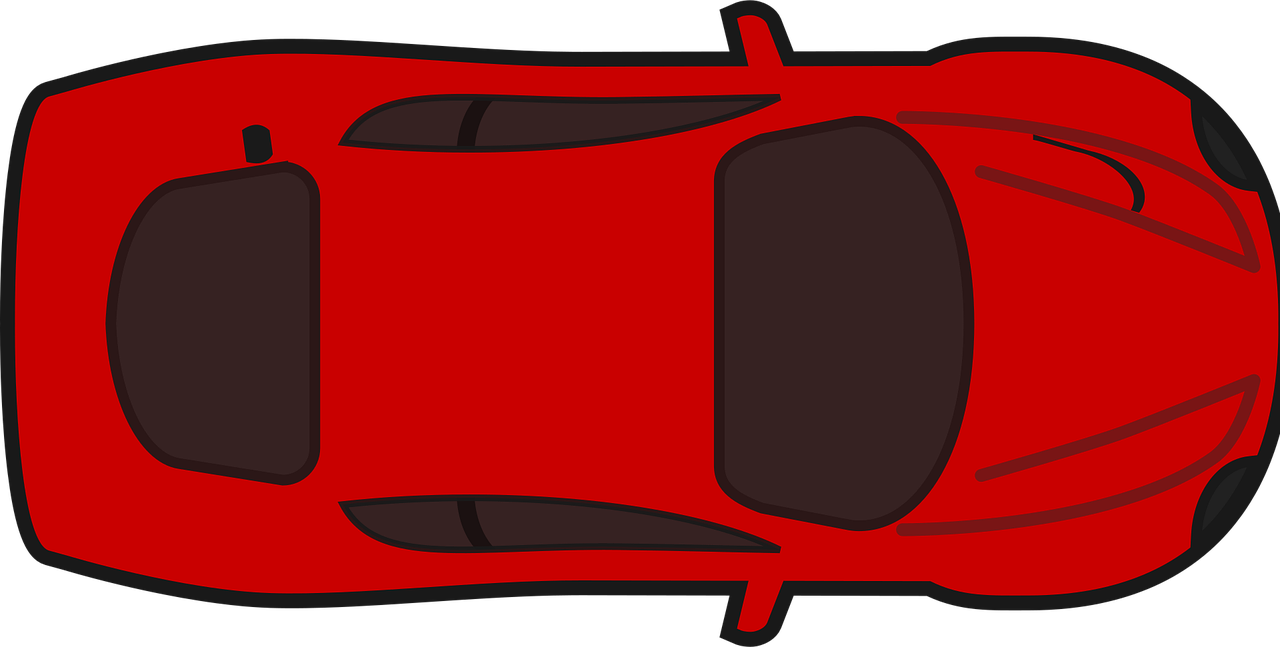
\includegraphics[width=\imgsize]{auto_bovenaan}};
        
        \fill[blue] (P\angle) circle (2pt);
        
        \draw[->, blue, very thick, -latex] 
        (P\angle) --++ (\angle+90:\vlength)
        node[thick, pos=0.6, font=\tiny, sloped, above] {$\vec{v}$};
        
        % Centripetal acceleration vector (toward center)
        \fill[xmgreen] (P\angle) circle (2pt);
        \draw[->, xmgreen, very thick, -latex] 
            (P\angle) -- ($(P\angle)!\alength!(center)$)
            node[thick, pos=0.8, font=\tiny, sloped, above] {$\vec{a}$};
    }
    
    \end{tikzpicture}
\end{image}
\end{example}

\begin{remark}
Combinatie van de twee types versnelling is ook mogelijk, bijvoorbeeld bij een schuin geworpen basketbal.
\begin{image}
	\begin{tikzpicture}[xscale=0.5, yscale=0.5]
		% \draw[thick,->] (0,0) -- (10,0) node[right] {$x$};
		% \draw[thick,->] (0,0) -- (0,10) node[above] {$y$};
	
		% \foreach \x in {1,...,10}
		%     \draw (\x,0) -- (\x,-0.2) node[below] {\x};
		% \foreach \y in {1,...,10}
		%     \draw (0,\y) -- (-0.2,\y) node[left] {\y};
		
		% Projectile parameters
		\def\v{15}          % Initial speed
		\def\theta{45}     % Launch angle in degrees
		\def\g{25}       % Gravity
		\def\vel{1}      % length of velocity vector
		\def\hoogte{3}  
		\def\imgsize{0.5cm}   
	
		% Trajectory
		\draw[thick, orange, domain=0:10, samples=50, smooth, dotted] 
			plot (\x, {tan(\theta)*\x - ( \g / (2 * \v * \v * cos(\theta)^2) ) * (\x)^2 + \hoogte});
		
		% Ball positions + velocity vectors in a single loop
		\foreach \x in {1,3,...,9} {
	
	
			% y-coordinate
			\pgfmathsetmacro{\y}{tan(\theta)*\x - ( \g / (2 * \v * \v * cos(\theta)^2) ) * (\x)^2 + \hoogte}
			% derivative (slope)
			\pgfmathsetmacro{\slope}{tan(\theta) - (\g / (\v*\v*cos(\theta)^2))*\x}
	
			\pgfmathsetmacro{\arrowHeadsize}{0.3*\vel} % you can replace with a more complex formula
	
	
			% Ball position (red dot or image)
			% \fill[red] (\x,\y) circle (1.5pt);
			\node at (\x,\y) {
\includegraphics[width=\imgsize]{basketbal}}; % optional
			
	
			\ifnum\x=9
			\else
			% Velocity vector tangent to trajectory
			% \draw[->, blue, very thick, -latex] (\x,\y) -- ++({\vel/sqrt(1+\slope*\slope)}, {\vel*\slope/sqrt(1+\slope*\slope)});
			\draw[->, blue, very thick, -latex] (\x,\y) -- ++(\vel, {\vel*\slope}) node[blue, pos=0.8, above]{\(\vec{v}\)};
			\fill[blue] (\x,\y) circle (2pt);
			
			\draw[->, xmgreen, very thick, -latex] (\x,{\y-0.2}) -- ++(0, -1) node[xmgreen, midway, left]{\(a\)};
			\fill[xmgreen] (\x,{\y-0.2}) circle (2pt);
			\fi
			
			\ifnum \x=9
			\node[xscale=-1, opacity=1] at ({\x+0.2},\y) {
\includegraphics[width=1cm]{basketring}}; 
			\fi
	
			}
		\end{tikzpicture}
			
\end{image}
\end{remark}

% \begin{remark}
% De zin van de snelheidsvector kan nooit plots veranderen omdat snelheid een grootheid is die enkel continu in de tijd kan veranderen. De zin van de snelheidsvector kan enkel wijzigen als de grootte van de snelheidsvector vermindert tot nul om dan nadien de tegengestelde zin uit te wijzen. In dit geval gaat het hier dus eveneens over de tangentiële versnelling.
% \end{remark}

% Ben het niet eens met deze opmerking. Hoe de snelheidsvector verloop hangt af van welk model je gebruikt. We gebruiken heel veel situaties waarin de we snelheid discontinu behandelen. Zo laten we de snelheidsvector bij een bots instant van zin veranderen, zo je wilt zonder verandering van grootte. Je hebt dan een discontinu verloop voor de snelheid.

% \begin{image}
% 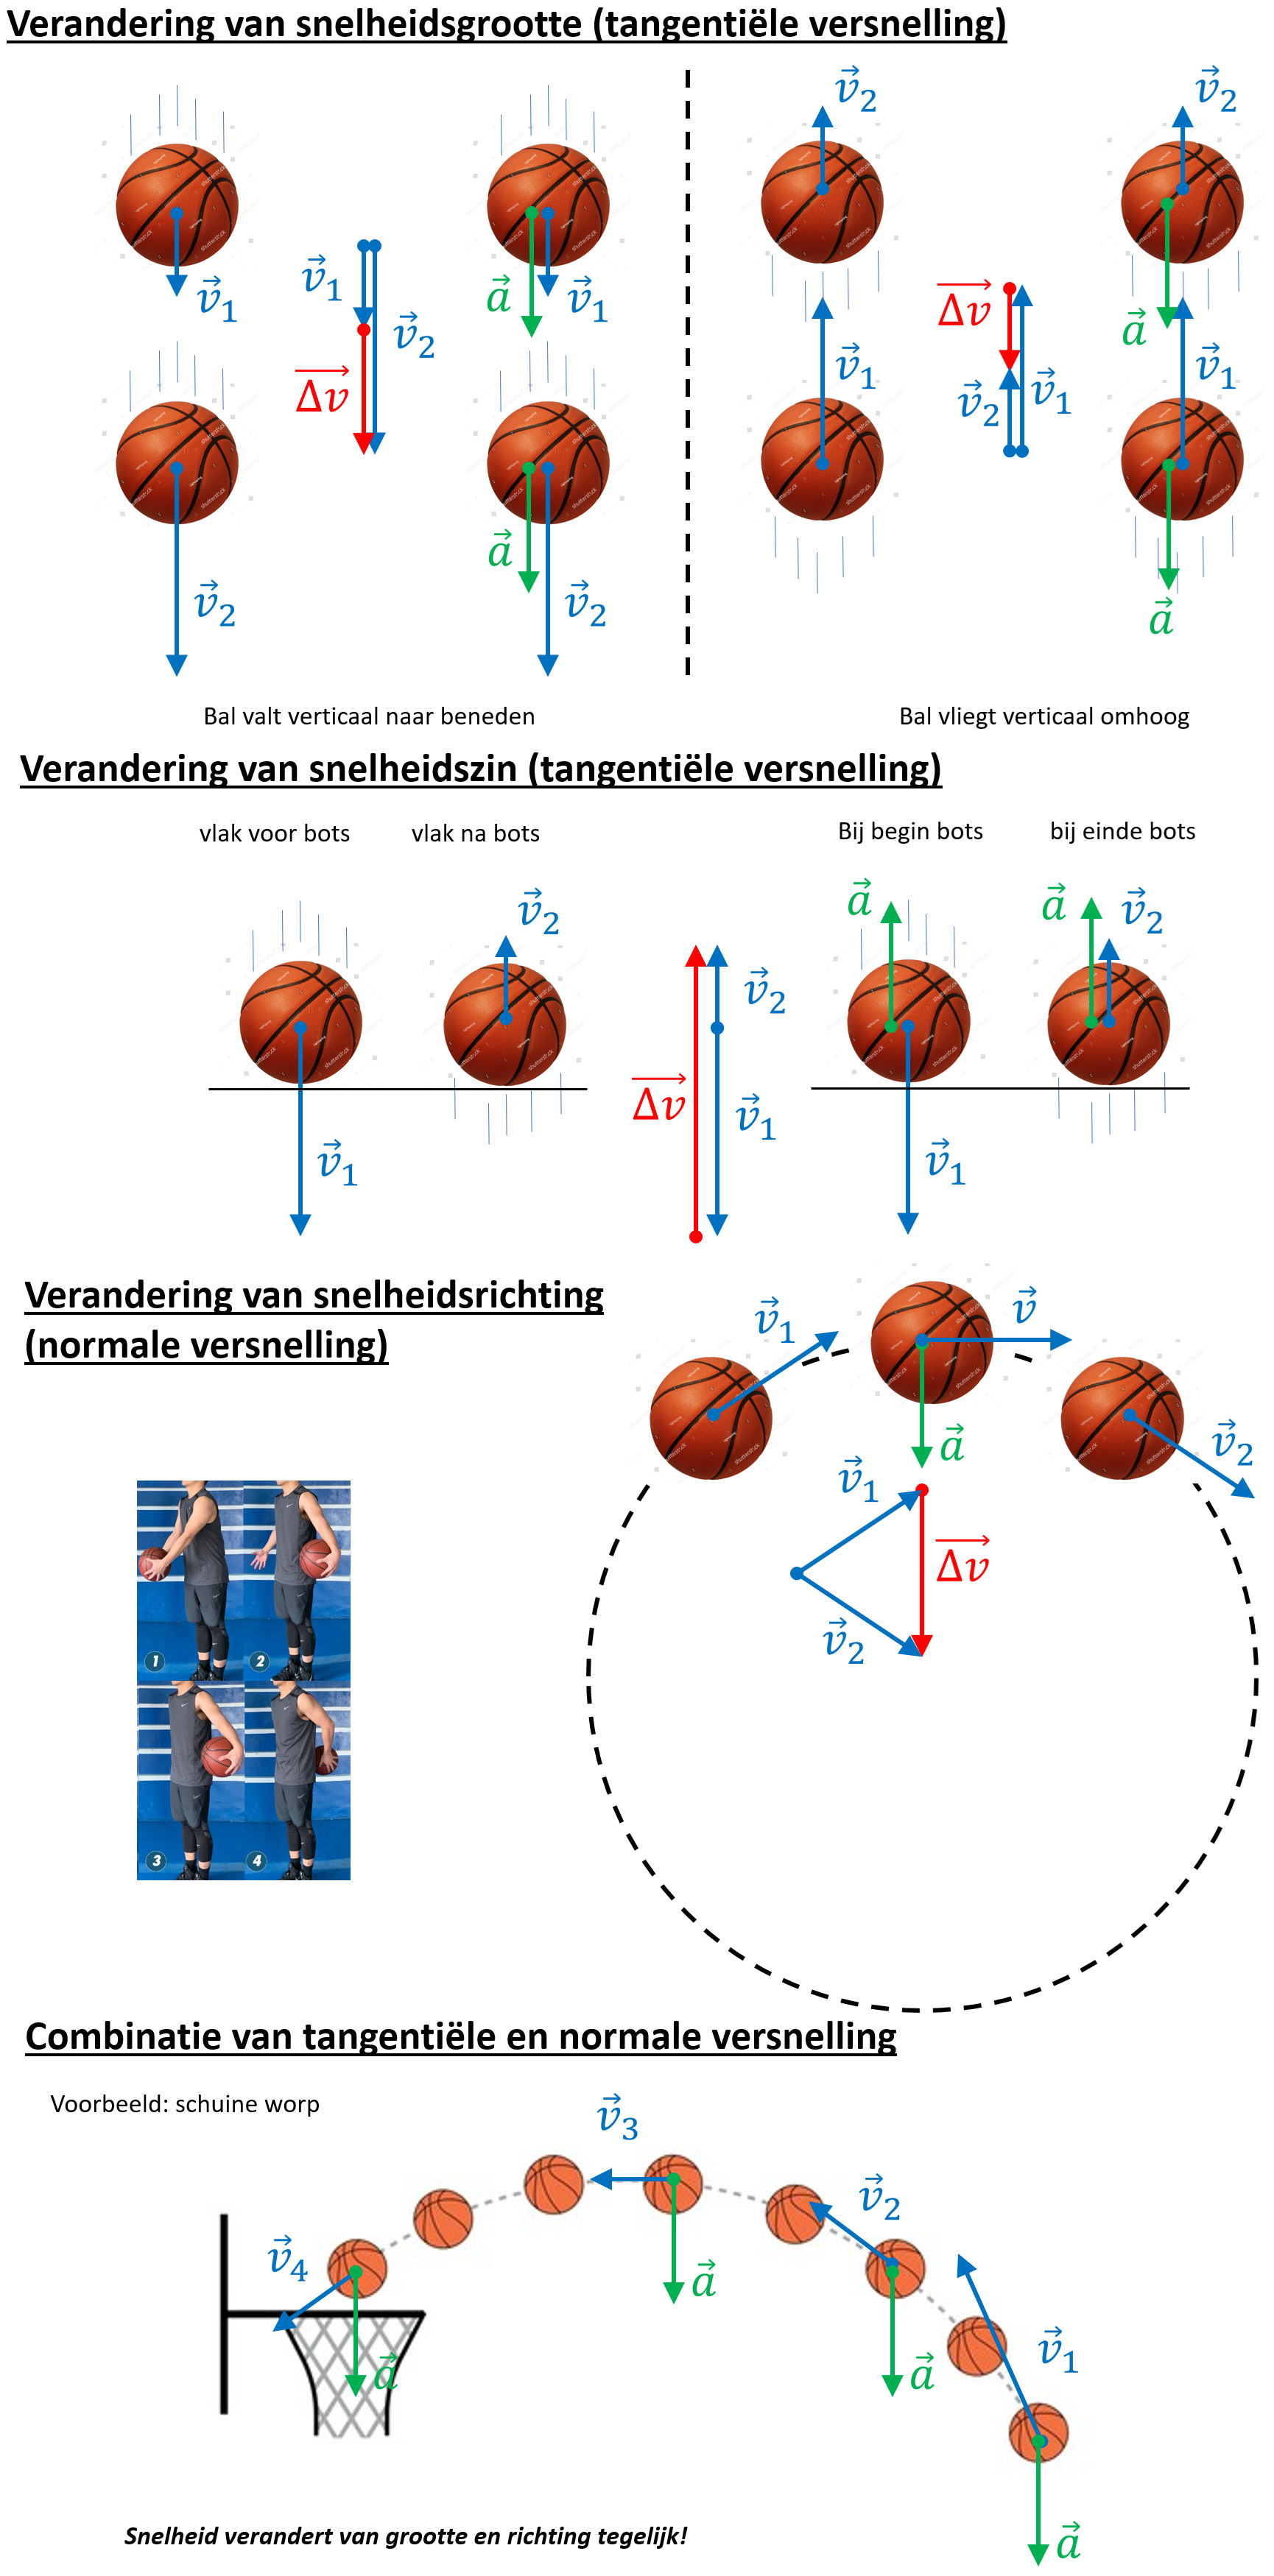
\includegraphics{soortenversnelling}
% \end{image}

% In al deze voorbeelden lijkt het alsof de versnellingsvector aan de snelheidsvector "trekt". = don't like this one ...

\subsection*{Gemiddelde versnelling bij eendimensionale bewegingen}
%\subsection*{Gemiddelde (tangentiële) versnelling bij eendimensionale bewegingen} = tangentieel is overbodig, want volgt uit het feit dat het eendimensionaal is. Scheermes van Ockham toegepast ... :-)

\begin{definition}

Bij eendimensionale bewegingen wordt de gemiddelde versnelling \(\overline{a}\) gedefinieerd als
\[
\overline{a}=\frac{\Delta v}{\Delta t}=\frac{v_2-v_1}{t_2-t_1}
\]
\end{definition}
%scalair gedefinieerd weggehaald. Je gaat niet naast een vectoriële ook een scalaire definitie installeren. Wat we volgens mij nu in de tekst wel aan het doen zijn. Moeten ergens aangeven dat we het over de component hebben.

% \begin{denkvraag*}{}
% Kan je uitleggen wat de eenheid meter per seconde, per seconde betekent? 
% \end{denkvraag*}
%%% Bizar: veroorzaakt [l.374] Missing number, treated as zero. at <to be read again> <- \c@depthICount

\subsection*{Ogenblikkelijke versnelling bij eendimensionale bewegingen}

De gemiddelde versnelling \(\overline{a}\) geeft de verandering in snelheid \textit{tussen} twee tijdstippen \(t_1\) en \(t_2\).  Om de ogenblikkelijke versnelling \(a\) op één tijdstip \(t\) te bepalen wordt -- net zoals bij de ogenblikkelijke snelheid -- gebruik gemaakt van de afgeleide.

\begin{definition}
	De ogenblikkelijke snelheid wordt gedefinieerd als de afgeleide van de snelheidsfunctie \(v(t)\):
	\[
		a=\lim_{t\to t_0}\frac{v(t)-v(t_0)}{t-t_0} = \frac{dv}{dt}=\frac{d^2x}{dt^2}
		\]
		De notatie met een accent $a(t)=v'(t)$ of $a=v'$ wordt op dezelfde manier als in de wiskunde gebruikt. $a(t)$ is een functie die op elk moment de versnelling geeft. 
	\end{definition}
	
	
	% Dit zijn erg drukke afbeeldingen 
	% \begin{image}
	% 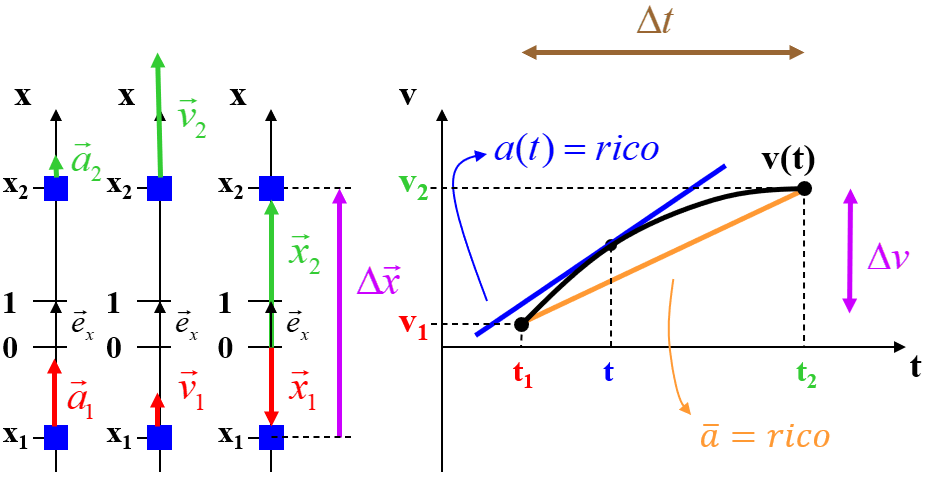
\includegraphics{versnellingmetgrafiek}
	% \end{image}

\subsection*{Ogenblikkelijke versnelling bij tweedimensionale bewegingen}
	
% In twee dimensies, kan men de versnelling opsplitsen in loodrechte x- en y-componenten. Daarmee kan men analoge redeneringen en gelijkaardige formules maken zoals in het 1D geval.
% is me niet heel duidelijk wat we hiermee zeggen ...
	
% \begin{image}
% 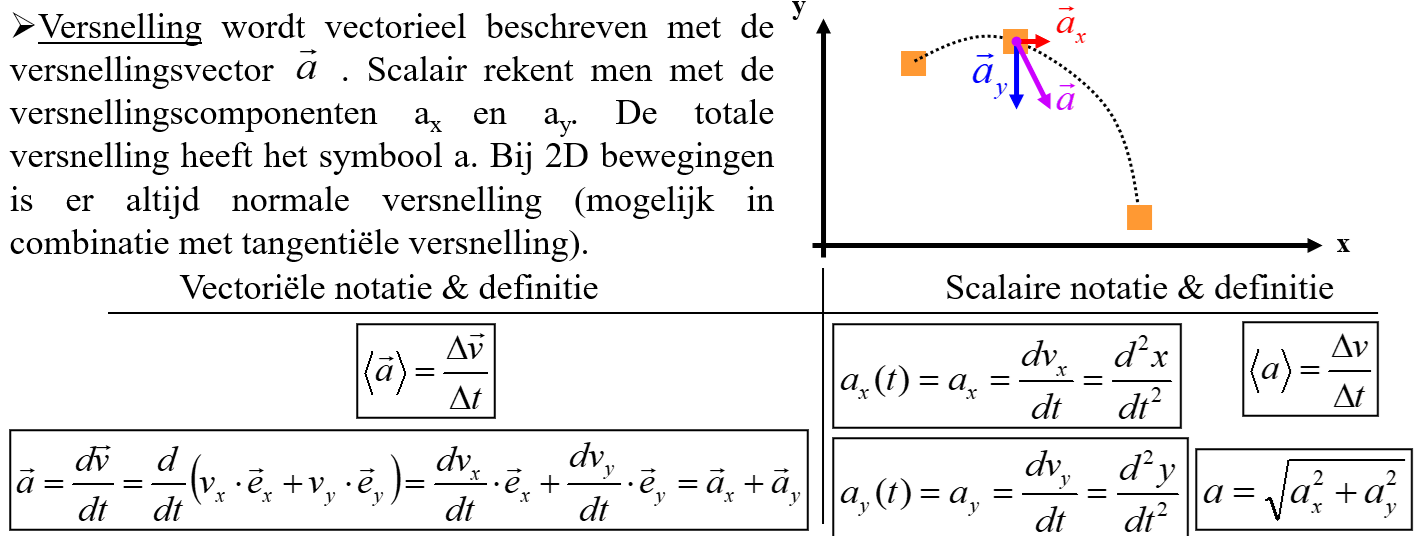
\includegraphics[width=0.8\textwidth]{versnelling2D}

% \end{image}
% BOVENSTAANDE SLIDE MET GPT NAAR TEX: 

% Versnelling wordt vectorieel beschreven met de versnellingsvector $\vec{a}$. 
% Scalair rekent men met de versnellingscomponenten $a_x$ en $a_y$. 
% De totale versnelling heeft het symbool $a$. = vector van maken
% Bij 2D bewegingen is er altijd normale versnelling (mogelijk in combinatie met tangentiële versnelling). = niet altijd waar. Ook een rechte baan kan je in 2D beschouwen en die heeft geen normale component voor de versnelling

In twee dimensies kan de snelheid naast een verandering van grootte ook een verandering van richting hebben. Om die te beschrijven is een vector het aangewezen object.

\begin{definition}
	
	De \textbf{versnellingsvector \(\vec{a}\)} van een lichaam wordt gedefinieerd als de afgeleide van de snelheidsvector naar de tijd:
	\[
	\vec{a}(t) = \frac{d\vec{v}(t)}{dt},
	\]
	en kan worden opgesplitst in versnellingscomponenten \(a_x\) en \(a_y\):
	% het hoef niet noodzakelijk over een bewegend punt te gaan. punt = lichaam/object/puntmassa = kan ook stilstaan
	\[
		\vec{a} = \frac{d\vec{v}}{dt} = \frac{d}{dt}(v_x \cdot \vec{e}_x + v_y \cdot \vec{e}_y) = \frac{dv_x}{dt} \cdot \vec{e}_x + \frac{dv_y}{dt} \cdot \vec{e}_y = a_x\cdot\vec{e}_x + a_y\cdot\vec{e}_y
	\]
	De grootte van de versnelling wordt genoteerd met het symbool \(a\) en is gelijk aan 
	\[
	a = \| \vec{a}\| = \sqrt{a_x^2 + a_y^2}
	\]
	
	\begin{image}[0.5\textwidth]
		\begin{tikzpicture}
			\draw[->] (-0.5,0) -- (3,0) node[right] {$x$};
			\draw[->] (0,-0.5) -- (0,3) node[above] {$y$};
			\coordinate (O) at (0,0);
	
			\pgfmathsetmacro{\r}{3}       
			\pgfmathsetmacro{\ang}{45} 
	
			\coordinate (A) at (\ang :\r);
	
			\fill (A) circle (2pt);
		
			\draw[->, very thick, blue, -latex] (O) -- (A) node[midway, below right] { $\vec{r}$};
	
			% Versnellingsvector tekenen
			\draw[->, very thick, xmgreen, -latex] 			(A) --++ (1, -1) node[pos=0.8, right, xshift=6pt]{ $\vec{a}$ versnellingsvector};
			\draw[->, very thick, xmgreen, dotted, -latex] 	(A) --++ (1, 0) node[midway, above right] { $\vec{a}_x$};
			\draw[->, very thick, xmgreen, dotted, -latex] 	(A) --++ (0, -1) node[pos=0.8, left ] { $\vec{a}_y$};
	
			\draw[->, thick, red, transform canvas={shift={(-0.05,-0.05)}}] (O) -- (0.5,0) node[midway, below] {$\vec{e}_x$};
			\draw[->, thick, red, transform canvas={shift={(-0.05,-0.05)}}] (O) -- (0,0.5) node[midway, left] {$\vec{e}_y$};
		\end{tikzpicture}
	\end{image}
	\captionof{figure}{Een versnellingsvector \(\vec{a}\)}
		
	\end{definition}

% \begin{remark}
% 	In bovenstaande figuur werd `in het algemene geval' een versnellingsvector getekend als vector die aangrijpt op de puntmassa. 
% 	In de bewegingen die we zullen bestuderen zal de versnellingsvector veroorzaakt zijn door de zwaartekracht of trekkracht. 
% 	Bijgevolg is de richting verticaal of in de richting van de positievector.   

% 	\begin{image}
% 		\begin{tikzpicture}
% 			\draw[->] (-0.5,0) -- (3,0) node[right] {$x$};
% 			\draw[->] (0,-0.5) -- (0,3) node[above] {$y$};
% 			\coordinate (O) at (0,0);
	
% 			\pgfmathsetmacro{\r}{3}       
% 			\pgfmathsetmacro{\ang}{45} 
	
% 			\coordinate (A) at (\ang :\r);
	
% 			\fill (A) circle (2pt);
		
% 			\draw[->, very thick, blue, -latex] (O) -- (A) node[midway, below right] { $\vec{r}$};
	
% 			% Versnellingsvector tekenen
% 			\fill[xmgreen] ([yshift=3pt]A) circle (2pt);
% 			\draw[->, very thick, xmgreen, -latex] 			(A) --++ (0, -1) node[pos=0.8, right, xshift=6pt]{ $\vec{a}$ };
% 			% \draw[->, very thick, xmgreen, dotted, -latex] 	(A) --++ (1, 0) node[midway, above right] { $\vec{a}_x$};
% 			% \draw[->, very thick, xmgreen, dotted, -latex] 	(A) --++ (0, -1) node[pos=0.8, left ] { $\vec{a}_y$};
	
% 			\draw[->, thick, red, transform canvas={shift={(-0.05,-0.05)}}] (O) -- (0.5,0) node[midway, below] {$\vec{e}_x$};
% 			\draw[->, thick, red, transform canvas={shift={(-0.05,-0.05)}}] (O) -- (0,0.5) node[midway, left] {$\vec{e}_y$};

% 			\node at (2,4) {De versnelling door de zwaartekracht};
% 		\end{tikzpicture}
% 		\hspace{1cm}
% 		\begin{tikzpicture}
% 			\draw[->] (-0.5,0) -- (3,0) node[right] {$x$};
% 			\draw[->] (0,-0.5) -- (0,3) node[above] {$y$};
% 			\coordinate (O) at (0,0);
	
% 			\pgfmathsetmacro{\r}{3}       
% 			\pgfmathsetmacro{\ang}{45} 
	
% 			\coordinate (A) at (\ang :\r);
	
% 			\fill (A) circle (2pt);
		
% 			\draw[->, very thick, blue, -latex] (O) -- (A) node[midway, below right] { $\vec{r}$};
	
% 			% Versnellingsvector tekenen
% 			\fill[xmgreen] ([yshift=3pt]A) circle (2pt);
% 			\draw[->, very thick, xmgreen, -latex] ([yshift=3pt]A) --++ (-1, -1) node[pos=0.8, above left, xshift=6pt]{ $\vec{a}$ };
% 			% \draw[->, very thick, xmgreen, dotted, -latex] 	(A) --++ (-1, 0) node[midway, above right] { $\vec{a}_x$};
% 			% \draw[->, very thick, xmgreen, dotted, -latex] 	(A) --++ (0, -1) node[pos=0.8, left ] { $\vec{a}_y$};
	
% 			\draw[->, thick, red, transform canvas={shift={(-0.05,-0.05)}}] (O) -- (0.5,0) node[midway, below] {$\vec{e}_x$};
% 			\draw[->, thick, red, transform canvas={shift={(-0.05,-0.05)}}] (O) -- (0,0.5) node[midway, left] {$\vec{e}_y$};

% 			\node at (2,4) {De versnelling door de trekkracht};
% 		\end{tikzpicture}
% 	\end{image}
% \end{remark}
% SORRY om dit even weg te halen maar het is te specifiek (er zijn nog andere mogelijkheden) en met te veel kennis van de tweede wet van newton die nodig is; kracht en versnelling zijn recht evenredig ...

% Vectoriële notatie en definitie:
	
% \[
% \langle \vec{a} \rangle = \frac{\Delta \vec{v}}{\Delta t}
% \]

% \[
% \vec{a} = \frac{d\vec{v}}{dt} 
% = \frac{d}{dt}(v_x \cdot \vec{e}_x + v_y \cdot \vec{e}_y) 
% = \frac{dv_x}{dt} \cdot \vec{e}_x + \frac{dv_y}{dt} \cdot \vec{e}_y 
% = \vec{a}_x + \vec{a}_y
% \]

% Scalaire notatie ens definitie:

% \[
% a_x(t) = a_x = \frac{dv_x}{dt} = \frac{d^2x}{dt^2}
% \]

% \[
% a_y(t) = a_y = \frac{dv_y}{dt} = \frac{d^2y}{dt^2}
% \]

% \[
% \langle a \rangle = \frac{\Delta v}{\Delta t}
% \]

% \[
% a = \sqrt{a_x^2 + a_y^2}
% \]


\begin{remark}
	Het begrip versnelling in de fysica heeft niet dezelfde betekenis als hoe het begrip in de volksmond wordt gebruikt.
	\begin{description}
		\item[In de volksmond] 
			\begin{itemize}
				versnelling = vergroten van snelheid

				vertraging = verkleinen van de snelheid

				bocht maken = richtingsverandering van de snelheid
			\end{itemize}
		\item[In de fysica]
			versnelling = verandering van snelheid in eender welk opzicht
	\end{description}

	De versnelling in de fysica is de grootheid $\vec{a}$ zoals die hierboven gedefinieerd is. We spreken van een vertraging wanneer de grootte van de snelheid afneemt. Dat kan voorkomen wanneer de snelheid (wat een vector is) en de versnelling (wat dus ook een vector is) een tegengestelde zin hebben. Hebben ze dezelfde zin, dan versnelt het voorwerp.

	% Fysisch zal men dus nooit spreken over een vertraging. Het vergroten of verkleinen van de snelheid moet bij eendimensionale bewegingen tot uiting komen in de zin van de versnellingsvector ten opzichte van de zin van de snelheidsvector. Men kan dit ook zien aan het teken van de getalcomponent van de versnelling tegenover die van de snelheid.
	% Voor eendimensionale bewegingen geldt dat als \(\vec{v}\) en \(\vec{a}\) dezelfde zin hebben (of hun getalcomponenten eenzelfde teken hebben) dat de snelheid (in absolute waarde) vergroot. Bij tegengestelde zin (of teken) is er in absolute waarde een verkleining van de snelheid.

	% Fysisch zal men dus nooit spreken over een vertraging.  = toch wel, wanneer de grootte van de snelheid afneemt ..? De versnelling (als vector) en de snelheid (als vector) zijn dan tegengesteld

\end{remark}

\begin{remark}

Wagens en fietsen hebben ook versnellingen. 
Weet dat deze versnellingen nauwelijks iets te maken hebben met het fysisch begrip versnelling. 
Een auto die in derde versnelling met een constante snelheid van 50 km/h rechtdoor rijdt, versnelt bijvoorbeeld helemaal niet. 
Zijn versnelling is 0 m/s². 
Een juistere naam om de standen van de versnellingspook of de ketting weer te geven had eigenlijk “snelheid” geweest omdat de versnelling waarin je rijdt veel meer zegt over welke snelheid je hebt. 
Kleine versnellingen gebruik je voor kleine snelheden en grote versnellingen voor grote snelheden. 
Onze Franstalige zuiderburen hebben daar een logischere naam voor, namelijk: “vitesse” (= snelheid). 
Probeer dus de begrippen snelheid en versnelling niet door elkaar te gooien, want ze hebben een heel andere betekenis! 
Het is alsof je zou zeggen dat positie en snelheid hetzelfde is!


\end{remark}

\begin{exercise}
Verklaar onderstaande meme. 

\begin{image}
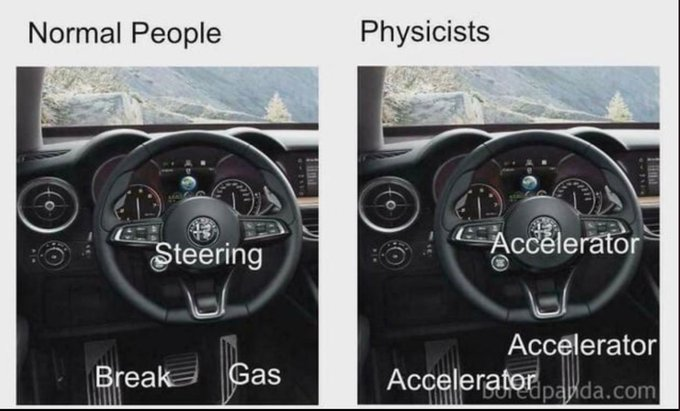
\includegraphics{meme_versnelling}
\end{image}

\end{exercise}
	
\end{document}